%%%%%%%%%%%%%%%%%%%%%%%%%%%%%%%%%%%%%%%%%
% Journal Article
% LaTeX Template
% Version 1.3 (9/9/13)
%
% This template has been downloaded from:
% http://www.LaTeXTemplates.com
%
% Original author:
% Frits Wenneker (http://www.howtotex.com)
%
% License:
% CC BY-NC-SA 3.0 (http://creativecommons.org/licenses/by-nc-sa/3.0/)
%
%%%%%%%%%%%%%%%%%%%%%%%%%%%%%%%%%%%%%%%%%

%----------------------------------------------------------------------------------------
%	PACKAGES AND OTHER DOCUMENT CONFIGURATIONS
%----------------------------------------------------------------------------------------

\documentclass[twoside]{article}

\usepackage{lipsum} % Package to generate dummy text throughout this template

\usepackage[sc]{mathpazo} % Use the Palatino font
\usepackage[T1]{fontenc} % Use 8-bit encoding that has 256 glyphs
\linespread{1.05} % Line spacing - Palatino needs more space between lines
\usepackage{microtype} % Slightly tweak font spacing for aesthetics
\usepackage{graphicx}
\graphicspath{ {images/} }
\graphicspath{ {figures/} }

\usepackage[hmarginratio=1:1,top=32mm,columnsep=20pt]{geometry} % Document margins
\usepackage{multicol} % Used for the two-column layout of the document
\usepackage[hang, small,labelfont=bf,up,textfont=it,up]{caption} % Custom captions under/above floats in tables or figures
\usepackage{booktabs} % Horizontal rules in tables
\usepackage{float} % Required for tables and figures in the multi-column environment - they need to be placed in specific locations with the [H] (e.g. \begin{table}[H])
\usepackage{hyperref} % For hyperlinks in the PDF

\usepackage{lettrine} % The lettrine is the first enlarged letter at the beginning of the text
\usepackage{paralist} % Used for the compactitem environment which makes bullet points with less space between them

\usepackage{abstract} % Allows abstract customization
\renewcommand{\abstractnamefont}{\normalfont\bfseries} % Set the "Abstract" text to bold
\renewcommand{\abstracttextfont}{\normalfont\small\itshape} % Set the abstract itself to small italic text

\usepackage{titlesec} % Allows customization of titles
\renewcommand\thesection{\Roman{section}} % Roman numerals for the sections
\renewcommand\thesubsection{\Roman{subsection}} % Roman numerals for subsections
\titleformat{\section}[block]{\large\scshape\centering}{\thesection.}{1em}{} % Change the look of the section titles
\titleformat{\subsection}[block]{\large}{\thesubsection.}{1em}{} % Change the look of the section titles

\usepackage{fancyhdr} % Headers and footers
\pagestyle{fancy} % All pages have headers and footers
\fancyhead{} % Blank out the default header
\fancyfoot{} % Blank out the default footer
%%AH\fancyhead[C]{Running title $\bullet$ November 2012 $\bullet$ Vol. XXI, No. 1} % Custom header text
%%\fancyhead[C]{November 18th, 2014}
\fancyfoot[RO,LE]{\thepage} % Custom footer text

%----------------------------------------------------------------------------------------
%	TITLE SECTION
%----------------------------------------------------------------------------------------

\title{\vspace{-15mm}\fontsize{24pt}{10pt}\selectfont\textbf{Hadoop Poker: Machine Learning in Texas Hold'em}} % Article title

\author{
\large
\textsc{Adrienne Humblet, David Kasofsky}\\[2mm] 
\normalsize New York University \\ 
\date{}
\vspace{-5mm}
}


%----------------------------------------------------------------------------------------

\begin{document}

\maketitle{} % Insert title

\thispagestyle{fancy} % All pages have headers and footers

%----------------------------------------------------------------------------------------
%	ABSTRACT
%----------------------------------------------------------------------------------------

\begin{abstract}

\noindent {
Abstract to come...
} 

\end{abstract}

%----------------------------------------------------------------------------------------
%	ARTICLE CONTENTS
%----------------------------------------------------------------------------------------

\begin{multicols}{2} % Two-column layout throughout the main article text

\section{Introduction} 
The goal of this analytic is to extract and present information from online poker hand logs. Our analysis would be restricted to No Limit Texas Hold'em, the most popular form of online poker. A single poker site like PokerStars will easily play billions of hands per year and a professional player may play hundreds of thousands if not millions of hands a year. This data can be used for at least the following purposes:
If one gathers sufficient data about a specific player, patterns in that player's play may become identifiable and thus exploitable when playing against that player.
Identifying Profitable Strategies. By examining many hands, one can identify which strategies tend to be profitable. Some machine learning algorithm could be used here, e.g. probabilistic classification to come up with a strategy like ``in this case, fold 20 percent of the time and bet 80 percent of the time. Here we'd definitely like the machine learning algorithm to have access to the player statistics gathered in the first example. ``
By combining statistics about particular players, i.e. the results of the first analysis, with guidelines for profitable play, i.e. the results of the second analysis, one may be to able to evaluate a particular player and identify the strong and weak parts of that player's game.

% Dummy text

%------------------------------------------------

\section{Motivation}

Imperfect information.

%------------------------------------------------

\section{Related Work}

The University of Alberta Poker Research Group has published many papers related to our topic.
One such paper describes using a support vector machine to train a poker bot on post-flop strategy. Since this yielded effective results, our project aims to extend a similar SVM mechanism for pre-flop strategy. 

%------------------------------------------------

\section{Design}


\subsection{Sources}
We used two sources of poker data. Both came in different formats that we have normalized using Map Reduce. 
\begin{compactitem}
\item{Poker Hand History} Our first source is the private hand history of a professional poker player who kindly agreed to donate his data to us. 
\item{IRC Poker Database} Seven years of poker data has been scraped from a dozen IRC poker channels. 
\end{compactitem}

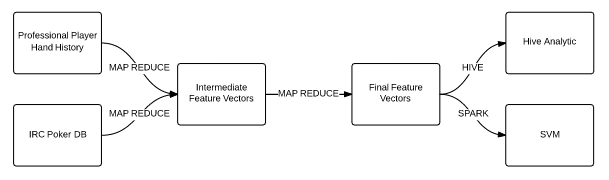
\includegraphics[scale=.5]{Flowchart.png}
Figure1.png


%------------------------------------------------

\section{Results}

%--------------------------------------------

\section{Future Work}

%------------------------------------------------

\section{Conclusion}

%------------------------------------------------

\section{Acknowledgements}

Many thanks to Jaime Staples for sending us his hand histories free of charge. 

%----------------------------------------------------------------------------------------
%	REFERENCE LIST
%----------------------------------------------------------------------------------------

\begin{thebibliography}{99} % Bibliography - this is intentionally simple in this template
\bibitem{counterpoint} F. Pachet. Musical Harmonization with Constraints: A Survey. Kluwer Publisher, 6(1):7-19, 2001.

\bibitem{computer composition} J. Moorer. Music and Computer Composition. Commun. ACM 15, 2. February 1972

\end{thebibliography}

%----------------------------------------------------------------------------------------

\end{multicols}

\end{document}
